\chapter{Selección de Instancias}
\label{capitulo1}
\lhead{Capítulo 1. \emph{Selección de Instancias}}

Este capítulo describe el problema de \emph{Selección de Instancias} (SI), como estrategia de reducción de datos para la aplicación de técnicas de \emph{Minería de Datos} (MD). El problema es definido formalmente, se describen sus principales características y se realiza un breve análisis del estado del arte.

\section{Reducción de Datos}

Como parte del proceso de \emph{Descubrimiento de Conocimiento en Bases de Datos} (Knowledge Discovery in Databases o \emph{KDD}), la fase de preprocesamiento de los datos juega un rol fundamental para la aplicación efectiva de técnicas de \emph{Minería de Datos} (\emph{MD}). Una de las estrategias de mayor uso durante la fase de preprocesamiento es la de \emph{reducción de datos}.

El problema de \emph{reducción de datos} consiste en decidir qué datos deben ser utilizados durante la aplicación de algoritmos de MD con el objetivo de construir modelos representativos de los datos originales. Dicha decisión debe basarse en la relevancia de los datos con respecto a los objetivos que se persiguen, o inclusive, por limitaciones técnicas. En términos prácticos, la importancia del problema de \emph{reducción de datos} radica en los siguientes factores:
\begin{inparaenum}[\itshape a\upshape)]
\item \textit{Tiempo y Espacio}: Mientras mayor sea el número de datos a utilizar, mayor será el espacio necesario para almacenarlos y el tiempo requerido para analizarlos. 
\item \textit{Sensibilidad al ruido}: Al aumentar el número de instancias en el conjunto de datos, también lo hace la probabilidad de aparición de datos atípicos, inconsistentes o redundantes. Su eliminación se vuelve necesaria para evitar un impacto negativo en los modelos de representación creados a partir de los datos.
\end{inparaenum}

En función de estos criterios, y basados en la definición de los datos, se han formulado diferentes estrategias para llevar a cabo la fase de reducción. En los procesos de KDD, un conjunto de datos está definido en función de un conjunto de clases $\Omega$ y un conjunto $T$ de $n$ observaciones de un evento, cada una con $m$ mediciones, donde:\\

\begin{definicion}
Una \textbf{instancia} $t_i$ (con $i = 1\dots n$) es una observación del evento; donde $t_i = (v_{i,1}, v_{i,2}, \dots, v_{i,m})$ es una tupla de $m$ valores/mediciones (un punto en un espacio $m$-dimensional). Adicionalmente, cada instancia $t_i$ pertenece a la \emph{clase} $\omega_{t_i} \in \Omega$.\\
\end{definicion}

\begin{definicion}
Un \textbf{atributo} $p_j$ (con $j = 1\dots m$) define el conjunto de mediciones \guillemotleft\emph{de un mismo tipo}\guillemotright\ para todas las observaciones, es decir, $p_j = \left\{ v_{i,j} \mid i = 1\dots n \right\}$. Cada atributo puede presentarse en diferentes formatos: \emph{nominales}, \emph{discretos}, o \emph{continuos}.
\end{definicion}

En la literatura se han definido varias estrategias para realizar el proceso de \emph{reducción de datos}. Entre ellas las más relevantes son:

\begin{itemize}
\item \textbf{Selección de Instancias}
\cite{DBLP:journals/ai/BlumL97,Liu:2002:IIS:593433.593525}: Busca la reducción del conjunto de datos mediante la selección de un subconjunto de instancias, de forma tal que dicho subconjunto conserve las capacidades de representación del conjunto original.
\item \textbf{Selección de Atributos}
\cite{DBLP:journals/ai/BlumL97, Liu:1998:FEC:551943}: Esta técnica permite eliminar atributos del conjunto de datos original, que no contribuyen (o que influyen negativamente) a la construcción de un modelo representativo.
\item \textbf{Discretización de Atributos}
\cite{DBLP:conf/ijcai/FayyadI93, Liu:2002:DET:593435.593535}: Esta estrategia busca convertir atributos \emph{continuos} en \emph{discretos} (cuantificando el espacio de posibles valores), o disminuir el número de valores \emph{discretos} (combinando valores adyacentes).
\end{itemize}

Digamos que se tiene una base de datos de pacientes en un hospital, y se desea entrenar un clasificador para predecir la existencia de enfermedades cardíacas en nuevos pacientes. Por cada paciente se registra su nombre, sexo, edad, altura, si es fumador o no, cuántas horas de ejercicio hace por semana, si tiene historia de enfermedades cardíacas en su familia, etc. Un algoritmo de selección de atributos eliminaría el atributo del nombre del paciente, puesto que no contribuye en la predicción esperada, mientras que siguiendo alguna estrategia de discretización de atributos, el atributo de edad podría dividirse en intervalos de 15 o 20 años. Finalmente, un algoritmo de selección de instancias buscará eliminar de la base de datos a pacientes con información faltante, repetidos o con valores fuera de lo común.

Este estudio se centra en el problema de \emph{Selección de Instancias}. En las siguientes secciones, el problema será definido formalmente y se describirán sus principales características.

\section{Selección de Instancias}

Dado un conjunto inicial de instancias $T = \left\{ t_i \mid i = 1 \dots n \right\}$ y un conjunto de clases $\Omega$, donde cada instancia está formada por una tupla de valores $t_i = (v_{i,1}, v_{i,2}, \dots, v_{i,m})$ y pertenece a la clase $\omega_{t_i}$, tal que $\omega_{t_i} \in \Omega$, el problema de \emph{Selección de Instancias} (SI) consiste en seleccionar un conjunto $R$, $R \subseteq T$, que mantenga (o mejore) la capacidad de representación del conjunto original $T$.

Este problema puede ser formulado como un \emph{problema de optimización combinatoria}, donde se busca el conjunto $R^*$, $R^* \subseteq T$, de menor cardinalidad que mantenga (o mejore) la capacidad de representación del conjunto original. Cada instancia perteneciente a $T$, puede o no pertenecer a $R$, lo que significa que el problema de SI tiene un espacio de posibles soluciones de cardinalidad igual a $2^n$.

En particular, la literatura se ha enfocado en la aplicación del problema de SI para su uso en clasificadores \cite{DBLP:journals/corr/GottliebK14,DBLP:conf/jcdcg/Toussaint02}. El subconjunto seleccionado se usa como conjunto de entrenamiento, en base al cual el clasificador estima la clase $\hat{\omega}$ de instancias previamente desconocidas. En este sentido, el problema de optimización de SI busca conseguir un conjunto $R^*$, $R^* \subseteq T$, \emph{consistente} y de cardinalidad mínima.\\

\begin{definicion}
Un conjunto $R$ es \textbf{consistente} con $T$, \emph{si y solo si} toda instancia $t \in T$ es clasificada correctamente (esto es, $\hat{\omega}_t = \omega_t$) mediante el uso de un clasificador \emph{M} y las instancias en $R$ como conjunto de entrenamiento.
\end{definicion}

La complejidad del problema de selección de instancias ha sido estudiada por diferentes autores: \emph{Bien} y \emph{Tibshirani} \cite{2012arXiv1202.5933B} describen una reducción del problema de SI al problema de \emph{Conjunto de Cobertura}, cuya versión de optimización es NP-Dura. Más aún, \emph{Wilfong} \cite{Wilfong:1991:NNP:109648.109673} y  \emph{Zukhba} \cite{Zukhba:2010:NPP:1921730.1921735} muestran que el problema de SI es NP-Duro.

En general, la literatura relacionada con el problema de SI se ha enfocado en el uso de clasificadores $k$-NN \cite{Garcia:2012:PSN:2122272.2122582} por su simplicidad y sobretodo, por su capacidad de representación de modelos sin información adicional sobre la distribución de los datos. El caso particular del problema de SI usando clasificadores $k$-NN también es conocido como \emph{Selección de Prototipos}. A continuación se describen estos clasificadores.

\subsection{Regla del Vecino Más Cercano (NN)}

Inicialmente descrita por \emph{Fix} y \emph{Hodges} \cite{fix_51_discriminatory}, la regla del \emph{Vecino Más Cercano} (Nearest Neighbor o NN) es una regla de inferencia basada en la idea de que instancias con atributos similares (cercanas en un espacio de $m$ dimensiones) tienden a compartir la misma clase. La regla NN estima la clase $\hat{\omega}_x$ de un punto $x$ en un espacio $m$-dimensional, dado un conjunto $R$ de instancias de entrenamiento y una función de distancia $\varphi$ entre dos puntos en dicho espacio:

\begin{equation}
\hat{\omega}_x = \omega_{t^*}\ ,\ 
t^* = \operatorname*{arg\,min}_{t\ \in\ R} \varphi(t,x)
\end{equation}

La generalización de la regla de inferencia NN se conoce como el clasificador $k$-NN: dado un $k \in \mathbb{N}$, se estima la clase $\hat{\omega}_x$ de un punto $x$ en función a la clase de las $k$ instancias más cercanas a $x$. En general, se usa la estrategia del \guillemotleft\emph{voto de la mayoría}\guillemotright, asignando la clase que más se repita entre las $k$ instancias más cercanas. En particular, el clasificador 1-NN corresponde a la regla NN.

$k$-NN es un clasificador no paramétrico de \emph{aprendizaje perezoso} (debido a que la etapa de aprendizaje consiste en guardar el conjunto de entrenamiento), caracterizado por su sencillez en términos de implementación. Esa simplicidad y su probada utilidad para numerosas aplicaciones, han hecho del clasificador $k$-NN uno de los más estudiados en la literatura.

Uno de los trabajos de mayor relevancia es el de \emph{Cover} y \emph{Hart} \cite{Cover:2006:NNP:2263261.2267456}, quienes mostraron que cuando el número de instancias de entrenamiento tiende a infinito, el clasificador $k$-NN garantiza un error no mayor al doble de la tasa de error de Bayes: la menor tasa de error posible para un clasificador dado. Adicionalmente, probaron que para un conjunto de entrenamiento de cardinalidad finita, el clasificador 1-NN es admisible dentro de la clase de clasificadores $k$-NN: es decir, no existe $k$, $k > 1$, tal que $k$-NN tenga menor probabilidad de error frente a 1-NN, para toda posible distribución de los datos.

Adicionalmente, algunos trabajos en geometría computacional han contribuido significativamente en la comprensión del problema. En este sentido, el clasificador 1-NN para espacios euclidianos puede definirse de forma alternativa en función de \emph{Diagramas de Voronoi} \cite{voronoi1908nouvelles}: una partición del espacio $\mathbb{R}^m$ en \emph{Celdas de Voronoi}, cada una definida por una instancia $t \in T$ donde $t$ es el \emph{vecino más cercano} para todos los puntos del espacio dentro de dicha celda (ver Figura \ref{voronoi}). Esto ha permitido el desarrollo de nuevos enfoques para la búsqueda de vecinos más cercanos basados en \emph{Diagramas de Voronoi}, como el descrito por \emph{Kolahdouzan} y \emph{Shahabi} \cite{Kolahdouzan:2004:VKN:1316689.1316762}.

\begin{figure}[h!]
\centering
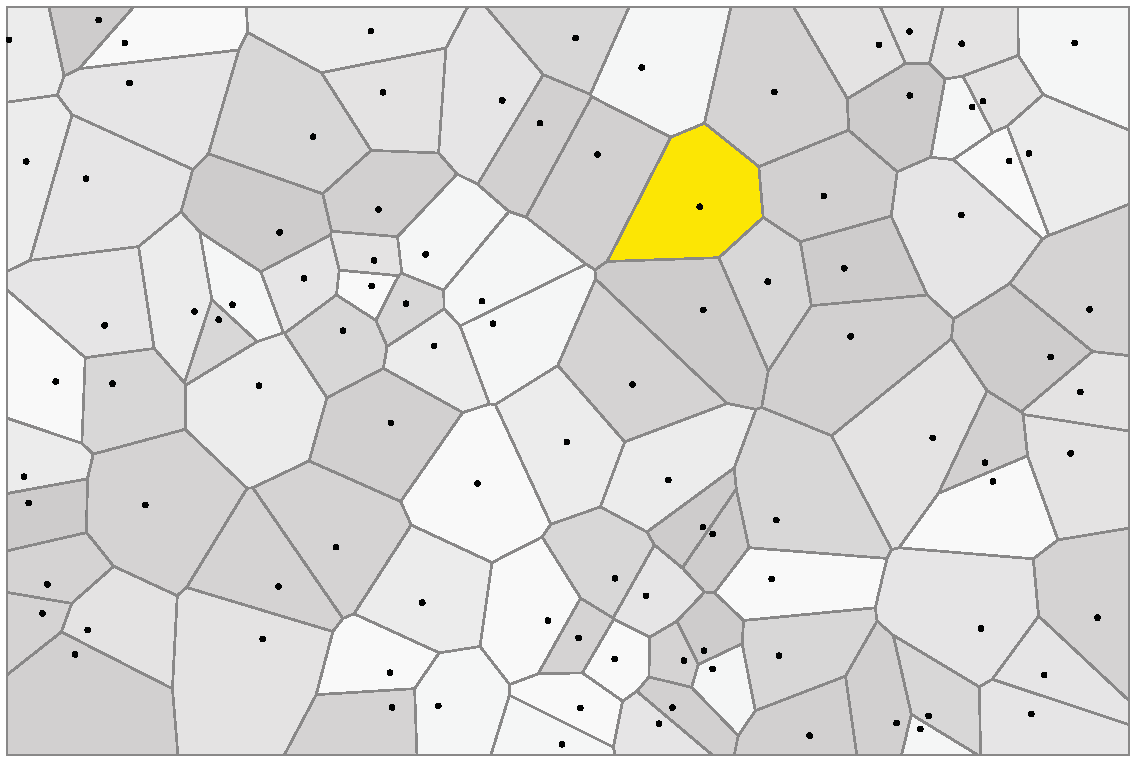
\includegraphics[width=0.6\textwidth]{voronoi.pdf}
\caption[Diagramas de Voronoi y NN]{Diagrama de Voronoi para instancias en un espacio $\mathbb{R}^2$. En amarillo la Celda de Voronoi de un punto $t \in T$, representando el espacio de puntos para los que $t$ es su \emph{vecino más cercano}.}
\label{voronoi}
\end{figure}

Similarmente, esta relación ha permitido avances importantes en términos de complejidad. En particular, mediante el uso de \emph{kd}-trees \cite{Bentley:1975:MBS:361002.361007} (árboles de búsqueda binaria en múltiples dimensiones) se ha logrado disminuir la complejidad en tiempo de clasificación, de $\mathcal{O}(n)$ (de un enfoque ``ingenuo'' revisando todas las instancias) a $\mathcal{O}(\log{n})$, a costa de un aumento en el tiempo necesario para el entrenamiento del clasificador: de $\mathcal{O}(1)$ a $\mathcal{O}(n\log{n})$, el tiempo necesario para la construcción del árbol.

Sin embargo, los clasificadores $k$-NN presentan ciertas propiedades desalentadoras; el problema de conseguir el vecino más cercano de un punto dado, requiere --en cualquiera de los casos-- almacenar todas las instancias de entrenamiento: $\mathcal{O}(n)$ en espacio. Adicionalmente, trabajos más recientes \cite{DBLP:conf/soda/KrauthgamerL04} muestran que en espacios euclidianos de altas dimensiones, la búsqueda del vecino más cercano requiere $\mathcal{O}(n)$ en tiempo: un fenómeno conocido como la \guillemotleft\emph{maldición de la dimensionalidad}\guillemotright\ (\emph{curse of dimensionality} en inglés). Finalmente, según \emph{Shwartz} y \emph{David} \cite{shalev2014understanding} los clasificadores NN tienden a sobre-ajustar el modelo con respecto al conjunto de entrenamiento (\emph{overfitting} en inglés); efecto que puede mitigarse aumentando el $k$ del clasificador \cite{devroye1994strong, shalev2014understanding} y eliminando instancias del conjunto de datos \cite{DBLP:journals/corr/GottliebKK13}.

\paragraph*{Algunas definiciones}
A continuación se definen algunos conceptos relevantes para la descripción de métodos heurísticos de SI en futuras secciones. Para un subconjunto cualquiera de instancias $Q$, $Q \subseteq T$:\\

\begin{definicion}
Los \textbf{asociados} en $Q$ de una instancia $t$ son aquellas instancias en $Q$ para las cuales $t$ pertenece a su conjunto de $k$ instancias más cercanas:
\begin{equation}
\emph{asociados}_Q(t) = \left\lbrace q \in Q \mid t\in \emph{kNN}(q) \right\rbrace
\end{equation}
\end{definicion}

\begin{definicion}
Los \textbf{enemigos} en $Q$ de una instancia $t \in T$ son aquellas instancias en $Q$ con una \emph{clase} diferente a la \emph{clase} de $t$:
\begin{equation}
\emph{enemigos}_Q(t) = \left\lbrace q \in Q \mid \omega_{q} \neq \omega_{t} \right\rbrace
\end{equation}
\end{definicion}

\begin{definicion}
El \textbf{enemigo más cercano} (\emph{nearest enemy} o NE) en $Q$ de una instancia $t \in T$, es la instancia más cercana a $t$ con diferente clase, y es denotada como $\mathrm{NE}_Q(t)$. Esto es, $\mathrm{NE}_Q(t)$ es la instancia más cercana a $t$ perteneciente a $\emph{enemigos}_Q(t)$:
\begin{equation}
\mathrm{NE}_Q(t) = \operatorname*{arg\,min}_{e\ \in\ \emph{enemigos}_Q(t)} \varphi(t,e)
\end{equation}
\end{definicion}

\section{Algoritmos de aproximación para Selección de Instancias}
\label{alg-aprox-si}

Debido a la complejidad del problema de SI, la literatura se ha enfocado en la definición de algoritmos heurísticos para conseguir soluciones aproximadas. De nuevo, el uso de clasificadores $k$-NN es una práctica extendida a lo largo de estos trabajos, por lo que las características de la regla NN han servido de inspiración para el desarrollo de la mayoría de los métodos de selección. Sin embargo, otras propuestas se basan en el orden de revisión de las instancias, así como en la realización de un muestreo aleatorio sobre el conjunto de datos. Finalmente, algunos enfoques se centran en aplicar procesos de búsqueda de propósito general, guiados por los objetivos del problema.

A continuación se describen brevemente algunos de los algoritmos heurísticos más recurrentes en la literatura relacionada al problema de SI.

\subsection{Métodos basados en la regla NN}

\begin{itemize}
\item \emph{Condensed Nearest Neighbor} (CNN) \cite{Hart:2006:CNN:2263267.2267647}\\
Inicialmente el conjunto $R$ se inicializa con una instancia cualquiera. Luego se itera sobre cada instancia $t \in T$; si $t$ no es clasificada correctamente usando $R$, $t$ se agrega a $R$.
CNN consigue un conjunto consistente, reduciendo considerablemente el conjunto de datos original. Sin embargo, no asegura un conjunto consistente mínimo, pues depende del orden en el que son revisadas las instancias en $T$.
\item \emph{Edited Nearest Neighbor} (ENN) \cite{wilson1972asymptotic}\\
Comienza con $R = T$. Luego itera sobre las instancias en $R$; aquellas que no sean bien clasificadas usando $R$ son eliminadas. Tiende a eliminar instancias ruidosas o cercanas a los bordes de decisión. Sin embargo, depende del orden en que itera sobre las instancias, y presenta bajas tasas de reducción dado que mantiene puntos internos.
\item \emph{Repeated Edited Nearest Neighbor} (RENN) \cite{wilson1972asymptotic}\\
Aplica ENN al conjunto de datos $R$ (inicialmente $R = T$) hasta que no ocurran cambios en $R$. Amplía la distancia entre clases y ``suaviza'' los bordes de decisión.
\item \emph{Reduced Nearest Neighbor} (RNN) \cite{DBLP:journals/tit/Gates72}\\
RNN extiende a CNN, usándola como solución inicial $R = R_{CNN}$. Luego, itera sobre cada instancia $t \in R$: si todas las instancias en $T$ son correctamente clasificadas usando $R\setminus\left\lbrace t \right\rbrace$, se elimina $t$ de $R$. En caso contrario, se mantiene $R$ y continua la iteración. La precisión de RNN puede mejorar respecto a CNN, pero es más costoso y su consistencia depende de la consistencia del conjunto resultante de CNN y del orden en que se iteren las instancias en $R$.
\end{itemize}

\subsection{Métodos basados en eliminación ordenada}

\begin{itemize}
\item \emph{Decremental Reduction Optimization Procedure 1} (DROP1) \cite{Wilson:1997:IPT:645526.657143}\\
Comienza con una solución inicial $R = T$. Itera sobre cada instancia $t \in R$: si todos sus \emph{asociados} en $R$ son correctamente clasificados con $R\setminus\left\lbrace t \right\rbrace$, $t$ se elimina de $R$. Reduce considerablemente el conjunto de datos inicial, pero obtiene baja precisión de clasificación, y el subconjunto resultante depende del orden en que se iteró sobre $T$.
\item \emph{Decremental Reduction Optimization Procedure 2} (DROP2) \cite{Wilson:1997:IPT:645526.657143}\\
Es una mejora sobre DROP1 en la cuál se elimina una instancia $t$ cuando todos sus \emph{asociados} en $T$ son clasificadas correctamente usando $R\setminus\left\lbrace t \right\rbrace$. Además, DROP2 ordena las instancias con respecto a la distancia de su \emph{enemigo} más cercano, en un intento de eliminar primero instancias centrales, y luego los puntos en los bordes de decisión.
\item \emph{Decremental Reduction Optimization Procedure 3} (DROP3) \cite{Wilson:1997:IPT:645526.657143}\\
Dado que el orden en que se iteran las instancias en DROP2 se ve alterado por puntos ruidosos, DROP3 filtra instancias ruidosas antes de ordenar el conjunto de entrenamiento.
\end{itemize}

\subsection{Métodos basados en muestreo aleatorio}

\begin{itemize}
\item \emph{Random Mutation Hill Climbing} (RMHC) \cite{DBLP:conf/icml/Skalak94}\\
Se selecciona un subconjunto de instancias aleatorias $R$ de tamaño fijo. En cada iteración el algoritmo intercambia una instancia en $R$ por una en $T \setminus R$; si el cambio mejora la precisión, se mantiene, en caso contrario se deshace.
\end{itemize}

\subsection{Métodos basados en metaheurísticas}

Las metaheurísticas son métodos de búsqueda estocástica de propósito general, usadas para encontrar soluciones óptimas o casi óptimas a problemas de optimización combinatoria. Por esta razón, muchos trabajos se han enfocado en el uso de estas técnicas para conseguir soluciones al problema de SI.

Algunos de los primeros trabajos se enfocaron en adaptar el algoritmo de \emph{Búsqueda Tabú} para solucionar el problema de SI. En particular, los estudios de \emph{Cerverón et al.} \cite{cerveron2001another} y \emph{Zhang et al.} \cite{zhang2002optimal} describen dos enfoques diferentes de modificación del algoritmo.

Sin embargo, la mayoría de los estudios se han enfocado en el uso de \emph{Algoritmos Evolutivos} (AE), adaptándolos para la búsqueda de soluciones al problema de selección. Entre ellos destaca el trabajo realizado por \emph{Cano et al.} \cite{cano2003using}; un completo estudio comparativo entre algoritmos ``tradicionales'' de SI y adaptaciones de \emph{Algoritmo Genético Generacional} (GGA), \emph{Algoritmo Genético Estacionario} (SGA), \emph{CHC Adaptive Search Algorithm} (CHC) y \emph{Population-Based Incremental Learning} (PBIL). Con este estudio, resulta evidente la utilidad de los \emph{AE} frente a los algoritmos tradicionales de SI en función de la capacidad de reducción y precisión de los conjuntos seleccionados.

Existen también otras adaptaciones y modificaciones sobre AE, entre los que destacan: \emph{Estimation of Distribution Algorithm} (EDA) \cite{sierra2001prototype}, \emph{Intelligent Genetic Algorithm} (IGA) \cite{ho2002design}, \emph{Steady-State Memetic Algorithm} (SSMA) \cite{garcia2008memetic} y \emph{Genetic Algorithm} \cite{gil2008evolving} basado en Error Cuadrático Medio, \emph{Clustered Crossover} y \emph{Fast Smart Mutation} (GA-MSE-CC-PSM).

%\subsection{Taxonomía}
%
%Debido a los numerosos enfoques existentes para aproximar soluciones al problema de SI, el trabajo de \emph{García} \emph{et al.} \cite{Garcia:2012:PSN:2122272.2122582} describe un esquema taxonómico para caracterizar las diferentes estrategias que se han desarrollado en base al uso de clasificadores $k$-NN. Dicho esquema clasifica las heurísticas de acuerdo al tipo de selección, y al tipo de evaluación y dirección de la búsqueda (ver Figura \ref{graphtaxonomia}).
%
%\begin{figure}[h!]
%\centering
%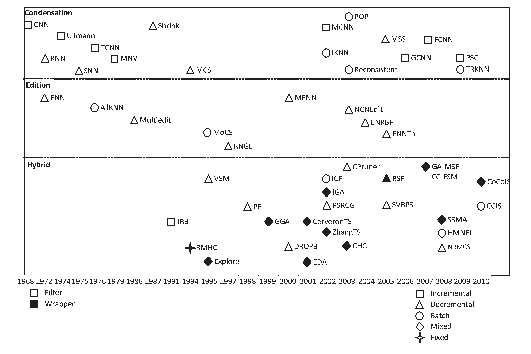
\includegraphics[width=0.7\textwidth]{taxonomia.pdf}
%\caption[Taxonomía de algoritmos de SI]{Taxonomía de algoritmos de aproximación\\para el problema de SI \cite{Garcia:2012:PSN:2122272.2122582}.}
%\label{graphtaxonomia}
%\end{figure}
%
%\noindent{\textbf{Según la dirección de la búsqueda}}\\
%La dirección en la cuál procede la búsqueda de posibles subconjuntos $R$ del conjunto inicial $T$ puede darse de diferentes formas.
%\begin{itemize}
%\item \emph{Incremental}:
%Comienzan con un conjunto $R$ vacio, o con unas pocas instancias representativas de cada clase en el conjunto de datos. En cada iteración se añaden nuevas instancias a $R$. Estos métodos tienden a ser más rápidos, pero dependen del orden de iteración sobre las instancias, y pueden producir un elevado \emph{overfitting}.
%\item \emph{Decremental}:
%Inicialmente $R = T$, y en cada iteración se eliminan elementos de $R$. Tienen la ventaja de contar inicialmente con todo el conjunto de datos para poder tomar decisiones, aunque son más costosos y dependen del orden de revisión de las instancias.
%\item \emph{Batch}:
%Estos métodos identifican aquellas instancias que cumplen cierto criterio, para luego eliminarlas/añadirlas todas como un conjunto. Presentan mayor complejidad.
%\item \emph{Mixed}:
%Comienzan con una selección aleatoria o con la selección dada por otro método de SI, para posteriormente añadir o eliminar instancias. Generalmente presentan \emph{overfitting}, además incrementar el tiempo de cómputo.
%\item \emph{Fixed}:
%Se refiere a una subcategoría de las heurísticas \emph{Mixed}, en la cuál se añaden y eliminan el mismo número de instancias; lo cuál no modifica el tamaño de la solución inicial.
%\end{itemize}
%
%\noindent{\textbf{Según el tipo de selección}}\\
%Varian en los tipos de instancias que seleccionan: puntos borde, centrales o cualesquiera.
%\begin{itemize}
%\item \emph{Condensation}:
%Seleccionan instancias cercanas a los bordes de decisión, también llamados puntos borde. Presentan mucha sencibilidad ante instancias ruidosas. En general estos métodos tienden a preservar la precisión para el conjunto de entrenamiento, pero afectan negativamente la generalización.
%\item \emph{Edition}:
%Buscan eliminar puntos borde para mantener bordes de decisión más ``suaves'', por lo que presentan menor sencibilidad ante puntos ruidosos. Tienden a mejorar la generalización del conjunto $T$ pero presentan un bajo porcentaje de reducción.
%\item \emph{Hybrid}:
%Permiten la selección de puntos borde y centrales con el objetivo de conseguir el menor conjunto $R$ que mantenga o aumente la precisión general del clasificador.
%\end{itemize}
%
%\noindent{\textbf{Según la evaluación de la búsqueda}}\\
%Diferentes estrategias para la evaluación de soluciones intermedias.
%\begin{itemize}
%\item \emph{Wrapper}:
%Utilizan el conjunto de datos completo sobre el clasificador\linebreak$k$-NN para la evaluación de soluciones intermedias, aplicando el esquema de validación \emph{leave-one-out}.
%\item \emph{Filter}:
%Usan solo partes del conjunto de datos original para la evaluación de soluciones intermedias, y sin aplicar el esquema de validación \emph{leave-one-out}. Implica menor tiempo evaluación, a costas de menor precisión.
%\end{itemize}

\subsection{Criterios de comparación}

Para comparar métodos de SI se consideran una serie de criterios usados para evaluar las ventajas y desventajas de cada algoritmo. A continuación se describen los factores más relevantes:

\begin{itemize}
\item \emph{Reducción}: El objetivo principal de métodos de SI es el de reducir el número de instancias del conjunto de datos. Esto no solo disminuye el espacio necesario para almacenar los datos, sino que acelera el proceso de clasificación.
\item \emph{Precisión}: Un algoritmo exitoso debe reducir el conjunto de datos, afectando en la menor medida posible su capacidad de generalización.
\item \emph{Tiempo}: A pesar de que el proceso de preprocesamiento y aprendizaje debe realizarse solo una vez, la complejidad de los algoritmos pueden volverlos poco prácticos para su uso sobre conjuntos ``grandes'' de datos.
\end{itemize}
